\chapter{Methods}\label{methods}

This chapter provides necessary background knowledge about the fundamental methods that are used in this thesis. First the main ideas behind the deep neural model that is used for paraphrase generation, are briefly explained. After that the learning strategies/approaches that are used in this work are explained.

\section{Recurrent Neural Networks}

\begin{figure}[t]
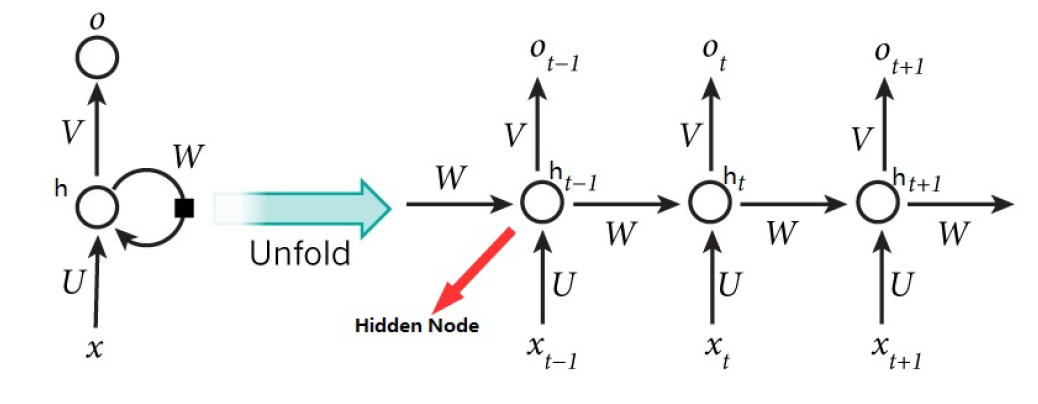
\includegraphics[width=\textwidth]{rnn}
\centering
\caption{Recurrent neural network expanding through time steps \cite{zhao}.}
\end{figure}

Recurrent neural networks (RNNs) are a type of neural network model designed for processing sequential data. The data is sequential which means it is processed in time steps by the model. This notion of time step does not have to mean literal concept of time that is used in real life. For example, it can be the position in the sequence (which is exactly the case for NLP). Since the length of a sequence can be really long, the model uses parameter sharing instead of optimizing separate parameters for each time step. This parameter sharing paradigm helps the model to generalize to different sequences by learning relationships between different time steps and different sequence lengths. Figure 2.1 shows a simple RNN and its expansion with respect to time. As it can be seen from the figure, the network produces an output in every time step.

Recurrent neural networks have numerous variants usually constructed by using different ways of connecting network layers or introducing additional computational mechanisms in order to increase generalization capability. 

\section{Long Short-Term Memory}

\begin{figure}[t]
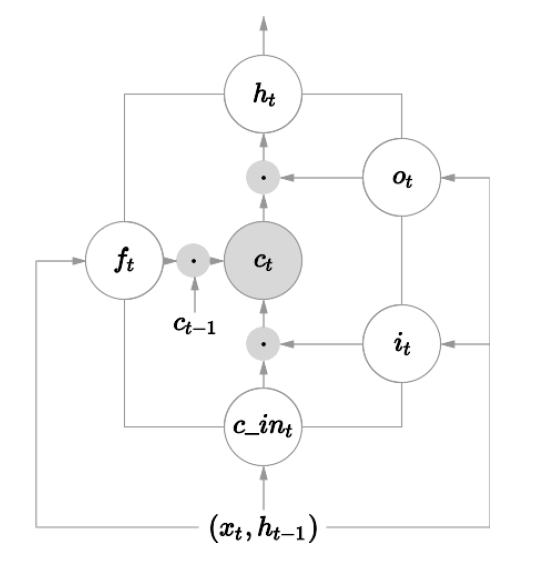
\includegraphics[scale=10]{lstm}
\centering
\caption{A typical LSTM cell \cite{paszke}.}
\end{figure}

Long Short-Term Memory (LSTM) is a variant of RNN that adds extra computational mechanisms to the network in order to avoid the vanishing and exploding gradient problems. These computational mechanisms include a memory cell and a set of logical gates. With these modifications, the model is able to remember information for long periods of time much better than vanilla RNNs.

Especially in NLP this is an important aspect since natural language contains context relationships, between words which can be observed at different time steps. 

LSTM adds a memory cell $c_{t}$ for every time step t. At each time step t, a single unit works with the input state $x_{t}$, the hidden state $h_{t-1}$ and the memory state $c_{t-1}$ to calculate the hidden state $h_{t}$ and the memory state $c_{t}$. The memory cell has three computational mechanisms: input gate i, forget gate f, and output o. These gates are also trained meaning that their weights are updates with gradient descent with respect to time. It is known that learning these gates helps with gradient explosion.

Figure 2.3 shows a basic LSTM cell. Equations for calculating the elements of an LSTM cell are \cite{paszke}:

\begin{equation}
i_{t} = \sigma(W_{xi}xt + W_{hi}h_{t-1} + b_{i})
\end{equation}

\begin{equation}
f_{t} = \sigma(W_{xf}xt + W_{hf}h_{t-1} + b_{f})
\end{equation}

\begin{equation}
o_{t} = \sigma(W_{xo}xt + W_{ho}h_{t-1} + b_{o})
\end{equation}

\begin{equation}
c_in_{t} = \tan(W_{xi}xt + W_{hi}h_{t-1} + b_{i})
\end{equation}

\begin{equation}
c_{t} = f_{t} \odot c_{t-1} + i_{t} \odot c_in_{t}
\end{equation}

\begin{equation}
h_{t} = o_{t} \odot \tan(c_{t}) 
\end{equation}

Parameters of the above equations are:

\begin{itemize}

\item $W_{x\_}$ and $W_{h\_}$: Weights for input x and hidden state h respectively.

\item $\sigma(\_)$ and $\tan(\_)$: Element-wise sigmoid function and hyperbolic tangent function.

\item $\odot$: Element-wise multiplication.

\item b: Bias parameter.

\end{itemize}

\section{Sequence to Sequence Model Architecture}

First introduced by \cite{Vinyalsetal} neural sequence to sequence framework consists of two components, encoder and decoder. Encoder creates a low dimensional representation of the source sequence called thought vector. It aims to capture semantical and contextual relationships of the source sequence. Thought vector then is fed into decoder which produces a high dimensional target sequence. The process is shown in Figure 2.1. Main idea of the encoder-decoder pair is to create a mapping between words and vectors, in other words capturing the meaning as numerical vectors. By design, both encoder and decoder should be a recurrent neural network or a variant of it. In the model that is used in this work, stacked LSTM's are used for both encoder and decoder. During the decoding process, generation of new words depends on the word generated before by decoder. The decoder starts generating the target sequence when it recognizes the 'EOS' (end-of-sentence) character in the source sequence. EOS character is usually appended to the end of source sequence. The model maximizes the log probability of the target sequence given the source sequence.

\begin{figure}[t]
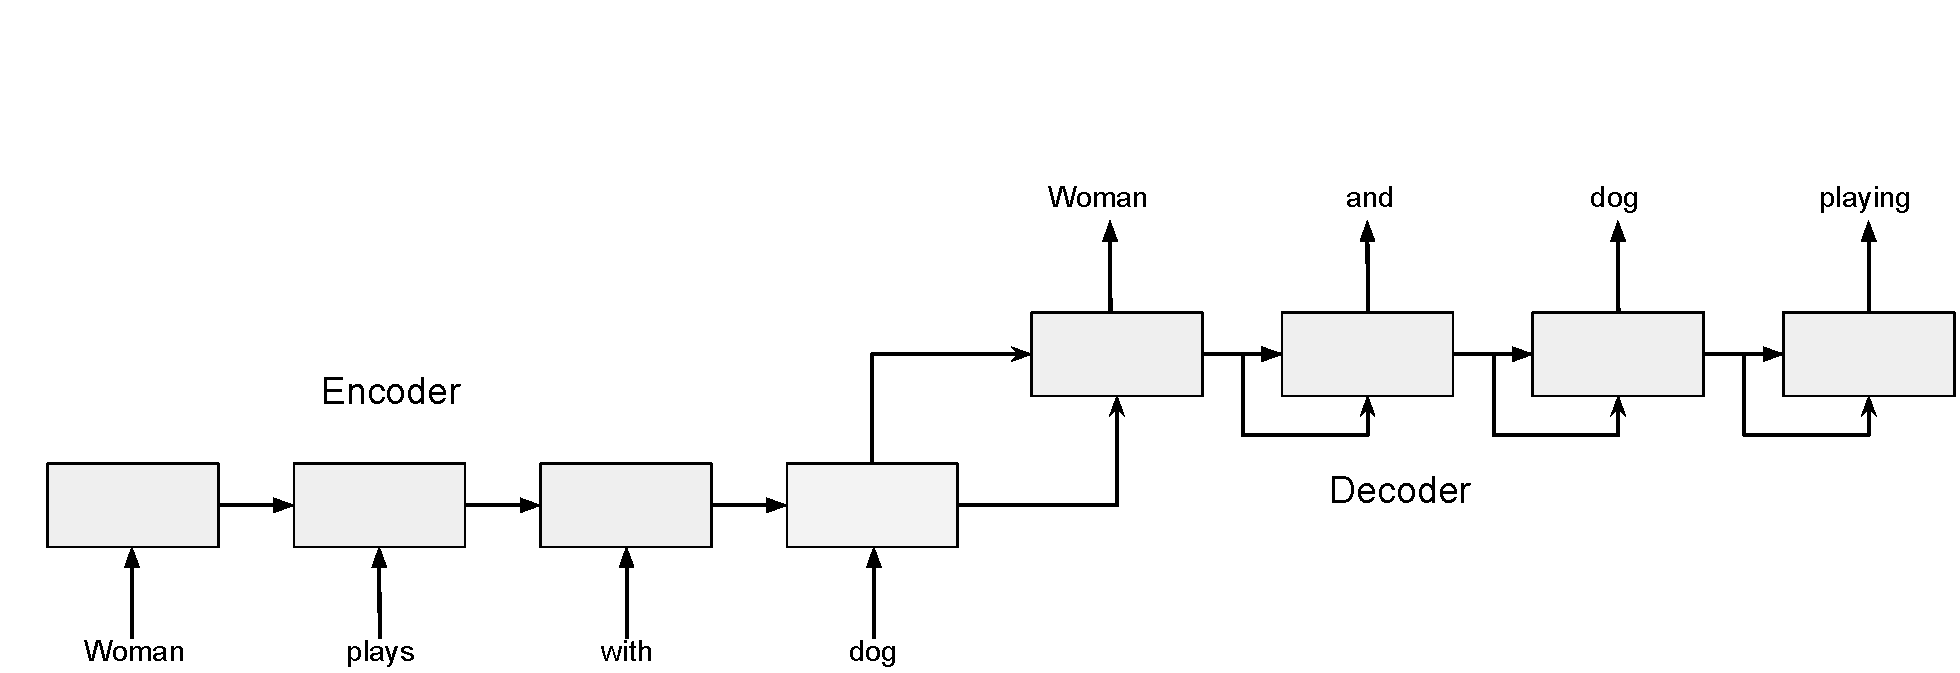
\includegraphics[scale=0.45]{seq2seq}
\centering
\caption{Sequence to sequence learning with encoder-decoder framework.}
\end{figure}

\section{Incremental Learning}

Incremental learning is a learning scheme based on training the model continuously in order to adapt to new training data without losing existing knowledge base. It is mainly used in cases where there is a data stream, constantly providing new data points. Incremental learning based models are mainly used to tackle problems like data availability and low resources. Incremental learning becomes essential in human-in-the-loop settings where the model has a feedback loop with users. Main concern of incremental learning is adaptivity since the model is especially prone to changes in training data distribution, a situation called concept drift which is explained in previous section. 

Additionally the specification of how to adapt the model creates another problem. Depending on the task and data at hand, how the model should exactly deal with the balance between old and new information has to be decided beforehand. Many incremental learning strategies for deep neural models consists of design decisions (hyper-parameters, network topology etc.) in order to deal with this problem. For example, using a large learning rate can lead the model to quickly overwrite existing knowledge with most recent data points. In this work, some of these strategies are experimented on paraphrase generation task.

\begin{figure}[t]
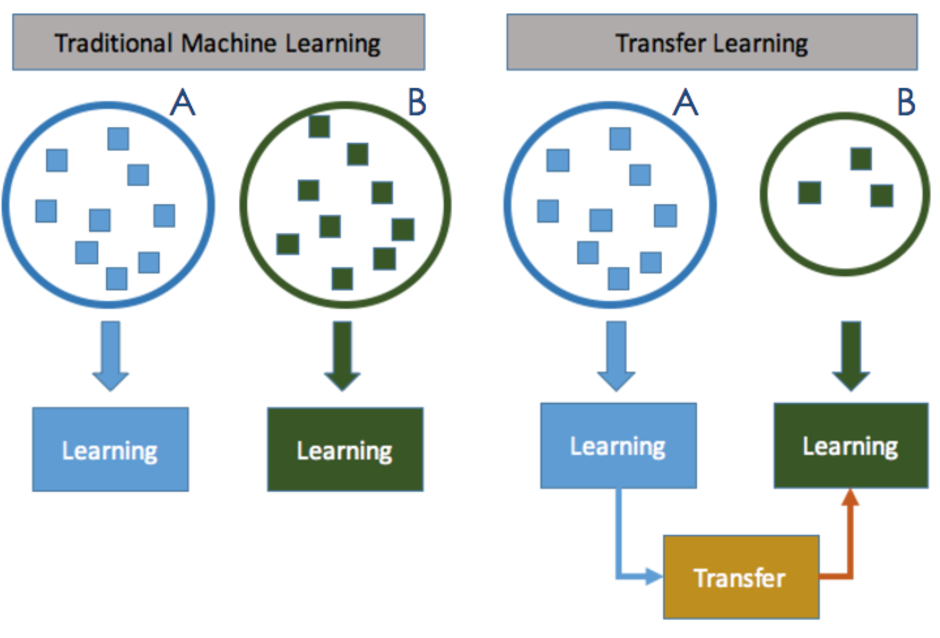
\includegraphics[width=\textwidth, height=10cm]{transfer-learning}
\centering
\caption{Idea behind transfer learning.}
\end{figure}

\section{Transfer Learning}

Transfer learning is based on the idea of using the knowledge gained from previously learned tasks and datasets. Usually it is used for decreasing the amount of training data and time of a low resource task where obtaining more training data is impractical. Moreover it is used for enhancing the recognition capabilities of an existing model, for example adding a new label for classification in image recognition task. This is a very important use case especially if the existing model is large since transferring knowledge eliminates the need of retraining the whole model. It can be also used to personalize an existing large model with a new domain specific dataset, enhancing its performance on the new domain. Figure 2.4 shows the basic workflow of transfer learning.

Deep neural models learn multiple hidden representations of the datasets, some part of which are shared between different tasks and datasets. Therefore transfer learning for deep neural models usually consists of copying layer weights across models and applying restrictions to new model in order to preserve existing knowledge. In the field of NLP, this process includes transferring learned word embeddings (numerical representations of words) and hidden layers (learned relationships of the datasets like context). Depending on the target task and dataset, the method of transfer which basically represents how the target model is trained, can significantly change. Different methods of transfer can include changing hyperparameters, freezing network layer or adding new layers.

\section{Active Learning}

Active learning is a learning scheme based on selecting training samples to be annotated by using different sampling strategies. These strategies employ certain criteria in order to create an opinion on how informative or useful a data point is and they are called sampling methods. Informativeness of a data point can depend on dataset, task and model therefore selection of the sampling method is very crucial. The criteria considered by a certain sampling method could simply be a heuristic about the nature of dataset at hand or they can depend on the opinion of model about the data points or they can depend on feature representations of the dataset like similarity measures. Usually, sampling methods combine multiple criterions for evaluating the informativeness of a data point and some of these criteria may require complex algorithms to be obtained. 

\begin{figure}[t]
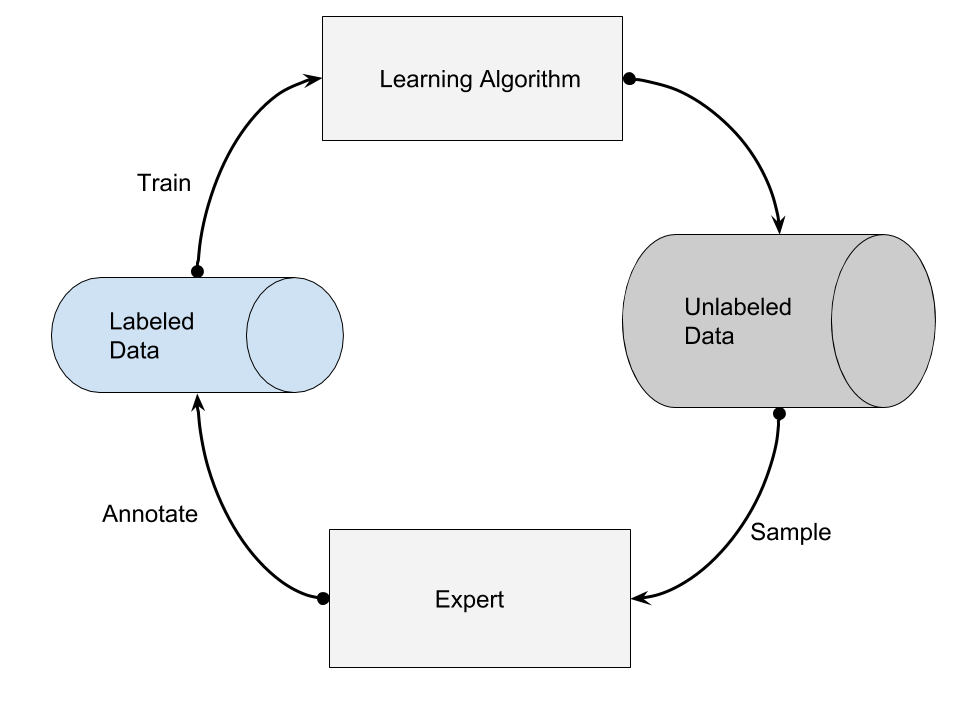
\includegraphics[width=\textwidth, height=10cm]{active-learning}
\centering
\caption{Pool based active learning scheme.}
\end{figure}

Figure 2.5 shows the basic workflow of active learning scheme. Main purpose of active learning is obtaining greater or similar performance with fewer labeled training data since collecting a large, labelled training data can be difficult, costing time and money. In our work, active learning is used as an option for enhancing human-in-the-loop data acquisition by asking the users to annotate most difficult samples. Additionally it is important to see if using adaptive learning can make the model more adaptive. It is also worth studying what constitutes an informative sample when it comes to paraphrase pairs.